\documentclass[final]{beamer}\usepackage[]{graphicx}\usepackage[]{color}
%% maxwidth is the original width if it is less than linewidth
%% otherwise use linewidth (to make sure the graphics do not exceed the margin)
\makeatletter
\def\maxwidth{ %
  \ifdim\Gin@nat@width>\linewidth
    \linewidth
  \else
    \Gin@nat@width
  \fi
}
\makeatother

\definecolor{fgcolor}{rgb}{0.345, 0.345, 0.345}
\newcommand{\hlnum}[1]{\textcolor[rgb]{0.686,0.059,0.569}{#1}}%
\newcommand{\hlstr}[1]{\textcolor[rgb]{0.192,0.494,0.8}{#1}}%
\newcommand{\hlcom}[1]{\textcolor[rgb]{0.678,0.584,0.686}{\textit{#1}}}%
\newcommand{\hlopt}[1]{\textcolor[rgb]{0,0,0}{#1}}%
\newcommand{\hlstd}[1]{\textcolor[rgb]{0.345,0.345,0.345}{#1}}%
\newcommand{\hlkwa}[1]{\textcolor[rgb]{0.161,0.373,0.58}{\textbf{#1}}}%
\newcommand{\hlkwb}[1]{\textcolor[rgb]{0.69,0.353,0.396}{#1}}%
\newcommand{\hlkwc}[1]{\textcolor[rgb]{0.333,0.667,0.333}{#1}}%
\newcommand{\hlkwd}[1]{\textcolor[rgb]{0.737,0.353,0.396}{\textbf{#1}}}%

\usepackage{framed}
\makeatletter
\newenvironment{kframe}{%
 \def\at@end@of@kframe{}%
 \ifinner\ifhmode%
  \def\at@end@of@kframe{\end{minipage}}%
  \begin{minipage}{\columnwidth}%
 \fi\fi%
 \def\FrameCommand##1{\hskip\@totalleftmargin \hskip-\fboxsep
 \colorbox{shadecolor}{##1}\hskip-\fboxsep
     % There is no \\@totalrightmargin, so:
     \hskip-\linewidth \hskip-\@totalleftmargin \hskip\columnwidth}%
 \MakeFramed {\advance\hsize-\width
   \@totalleftmargin\z@ \linewidth\hsize
   \@setminipage}}%
 {\par\unskip\endMakeFramed%
 \at@end@of@kframe}
\makeatother

\definecolor{shadecolor}{rgb}{.97, .97, .97}
\definecolor{messagecolor}{rgb}{0, 0, 0}
\definecolor{warningcolor}{rgb}{1, 0, 1}
\definecolor{errorcolor}{rgb}{1, 0, 0}
\newenvironment{knitrout}{}{} % an empty environment to be redefined in TeX

\usepackage{alltt}
\usepackage{grffile}
\mode<presentation>{\usetheme{CambridgeUSPOL}}

\usepackage[utf8]{inputenc}
\usepackage{amsfonts}
\usepackage{amsmath}
\usepackage{natbib}
\usepackage{graphicx}
\usepackage{array,booktabs,tabularx}
\newcolumntype{Z}{>{\centering\arraybackslash}X}

% rysunki
\usepackage{tikz}
\usepackage{ifthen}
\usepackage{xxcolor}
\usetikzlibrary{arrows}
\usetikzlibrary[topaths]
\usetikzlibrary{decorations.pathreplacing}
%\usepackage{times}\usefonttheme{professionalfonts}  % times is obsolete
\usefonttheme[onlymath]{serif}
\boldmath
\usepackage[orientation=portrait,size=a0,scale=1.4,debug]{beamerposter}                       % e.g. for DIN-A0 poster
%\usepackage[orientation=portrait,size=a1,scale=1.4,grid,debug]{beamerposter}                  % e.g. for DIN-A1 poster, with optional grid and debug output
%\usepackage[size=custom,width=200,height=120,scale=2,debug]{beamerposter}                     % e.g. for custom size poster
%\usepackage[orientation=portrait,size=a0,scale=1.0,printer=rwth-glossy-uv.df]{beamerposter}   % e.g. for DIN-A0 poster with rwth-glossy-uv printer check
% ...
%

\usecolortheme{seagull}
\useinnertheme{rectangles}
\setbeamercolor{item projected}{bg=darkred}
% \setbeamertemplate{enumerate items}[default]
\setbeamertemplate{navigation symbols}{}
\setbeamercovered{transparent}
\setbeamercolor{block title}{fg=darkred}
\setbeamercolor{local structure}{fg=darkred}

\setbeamercolor*{enumerate item}{fg=darkred}
\setbeamercolor*{enumerate subitem}{fg=darkred}
\setbeamercolor*{enumerate subsubitem}{fg=darkred}

\setbeamercolor*{itemize item}{fg=darkred}
\setbeamercolor*{itemize subitem}{fg=darkred}
\setbeamercolor*{itemize subsubitem}{fg=darkred}

\newlength{\columnheight}
\setlength{\columnheight}{95cm}
\renewcommand{\thetable}{}
\def\andname{,}
\authornote{}

\renewcommand{\APACrefatitle}[2]{}
\renewcommand{\bibliographytypesize}{\footnotesize} 
\renewcommand{\APACrefYearMonthDay}[3]{%
  {\BBOP}{#1}
  {\BBCP}
}
\IfFileExists{upquote.sty}{\usepackage{upquote}}{}
\begin{document}






\date{}
\author{Micha\l{}  Burdukiewicz\inst{1}*, Piotr Sobczyk\inst{2}, Pawe\l{} Mackiewicz\inst{1}, Stefan R\"odiger\inst{3} \\
\small{*michalburdukiewicz@gmail.com}}

\institute{\small{\textsuperscript{1}University of Wroc\l{}aw, Department of Genomics

\vspace{0.2cm}

\textsuperscript{2}Wroc\l{}aw University of Technology, Faculty of Pure and Applied Mathematics

\vspace{0.2cm}

\textsuperscript{3}Brandenburg University of Technology Cottbus-Senftenberg, Institute of Biotechnology}

}
\title{\huge dpcR: web server and R package for analysis of digital PCR experiments}

\begin{frame}
  \begin{columns}
    \begin{column}{.46\textwidth}
      \begin{beamercolorbox}[center,wd=\textwidth]{postercolumn}
        \begin{minipage}[T]{.95\textwidth}
          \parbox[t][\columnheight]{\textwidth}
            {
    
        
    \begin{block}{Introduction}
      dPCR reaction consists of multiple amplifications occurring in numerous small partitions. The result of dPCR is a binary vector describing states of partitions (positive in case of detected amplification, negative otherwise). This data is further used to estimate the main parameter, $\lambda$, which may be interpreted as the mean number of template molecules per partition.
      
      We created dpcR, an open source tool for reproducible analysis of dPCR data, fully compatible with dMIQE requirements.
    \end{block}
    
    \vfill
    
    \begin{block}{dpcR workflow}

      \begin{figure}
\begin{center}
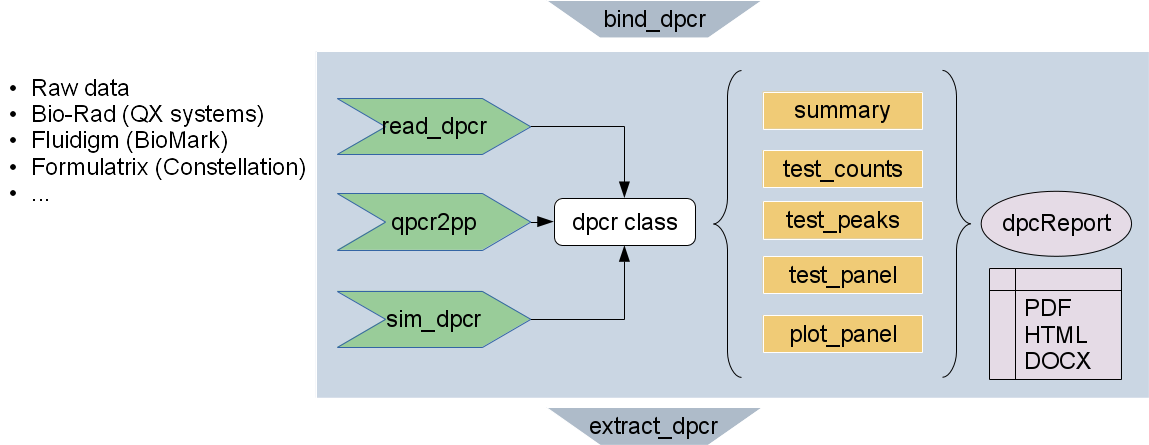
\includegraphics{figures/dpcR_framework.png}
\end{center}
\label{workflow}
\end{figure}

\textit{dpcR} workflow. The diagram shows main functions available at each step of a dPCR data analysis.

    \end{block}
    \vfill
    
    
    \begin{block}{Hidden semi-Markov model (HSMM) of a signal peptide}
      Assumptions of the model:
      \begin{itemize}
        \item the observable distribution of amino acids arises due to being in a certain region (state),
        \item a duration of the state (the length of given region) is modeled by a probability distribution (other than geometric distribution as in typical hidden Markov models).
      \end{itemize}
    \end{block}
    \vfill
            }
        \end{minipage}
      \end{beamercolorbox}
    \end{column}
    
    
%new column ------------------------------------------------------    
    
    \begin{column}{.54\textwidth}
      \begin{beamercolorbox}[center,wd=\textwidth]{postercolumn}
        \begin{minipage}[T]{.95\textwidth}  
          \parbox[t][\columnheight]{\textwidth}
            {
     
    \begin{block}{Conclusions}
      Hidden semi-Markov models can be used to accurately predict the presence of secretory signal peptides effectively extracting information from very data sets. Prediction of cleavage site position still requires refinement.
    \end{block}
    \vfill 
    
        \begin{block}{Availability and funding}
        \footnotesize{
      signal.hsmm web server: 
      
      \url{www.smorfland.uni.wroc.pl/signalhsmm}
        }
        
        This research was partially funded by KNOW Consortium.
    \end{block}
    \vfill 
     
     
    \begin{block}{Bibliography}
    \tiny{
      \bibliographystyle{apalike}
      \bibliography{amyloids}
    }
    \end{block}
    \vfill
            }
        \end{minipage}
      \end{beamercolorbox}
    \end{column}
  \end{columns}  
\end{frame}
\end{document}
